\documentclass[aspectratio=169, 10pt]{beamer}

% Theme & Color Palette (Standard Built-in Madrid Theme)
\usetheme{Madrid}
\usecolortheme{whale}
\usefonttheme{professionalfonts}

% Packages
\usepackage[utf8]{inputenc}
\usepackage{amsmath, amssymb, amsfonts}
\usepackage{booktabs}
\usepackage{tikz}
\usetikzlibrary{positioning, arrows.meta, calc, shapes.geometric}
\usepackage{graphicx}
\usepackage{hyperref}

% Custom Colors
\definecolor{mainblue}{RGB}{26, 54, 93}
\definecolor{secblue}{RGB}{43, 108, 176}
\definecolor{accentteal}{RGB}{49, 151, 149}
\definecolor{bglight}{RGB}{247, 250, 252}

\setbeamercolor{structure}{fg=mainblue}
\setbeamercolor{palette primary}{bg=mainblue, fg=white}
\setbeamercolor{palette secondary}{bg=secblue, fg=white}
\setbeamercolor{palette tertiary}{bg=accentteal, fg=white}
\setbeamercolor{titlelike}{bg=mainblue, fg=white}
\setbeamercolor{block title}{bg=secblue, fg=white}
\setbeamercolor{block body}{bg=bglight, fg=black}

% Metadata
\title[Sensor-Centric Traffic Framework]{An Intelligent Sensor-Centric Framework for Traffic Analysis and Forecasting}
\subtitle{Proposal Review \& Dissertation Presentation}
\author[Souptik Hazra \& Prof. K. Brindha]{Presented by: \textbf{Souptik Hazra} \\[0.2cm] Under the Guidance of: \textbf{Prof. K. Brindha}}
\institute[Department of Computer Science]{Department of Computer Science \& Engineering}
\date{\today}

\begin{document}

% ==================== SLIDE 1: TITLE ====================
\begin{frame}[plain]
  \titlepage
\end{frame}

% ==================== SLIDE 2: ABSTRACT ====================
\begin{frame}{Abstract}
  \begin{block}{Research Overview}
    Spatiotemporal Graph Neural Networks (ST-GNNs) forecast urban traffic dynamics across physical road sensor networks. Standard deep learning architectures optimize global loss functions, concealing severe spatial prediction error disparities between highway sub-networks.
  \end{block}

  \begin{block}{Proposed Framework}
    A 4-Layer Structural Causal Digital Twin framework evaluates and remediates regional prediction error disparities without sacrificing forecasting accuracy. By embedding Judea Pearl's Level-3 Structural Causal Model (SCM) into a virtual replica of physical highway sensors, the framework disentangles hardware sensor dropouts from true physical traffic jams using spatial neighborhood checks.
  \end{block}

  \begin{block}{Key Outcome}
    Establishes a mathematical foundation for identifying physical root causes of forecasting disparity, providing transportation authorities with actionable infrastructure maintenance decision support.
  \end{block}
\end{frame}

% ==================== SLIDE 3: CONTEXT ====================
\begin{frame}{1. Research Context \& Background}
  \begin{itemize}
    \item \textbf{Intelligent Transportation Systems (ITS):} Modern smart cities rely heavily on ITS for dynamic traffic control, route planning, and emergency response.
    \item \textbf{Spatiotemporal Traffic Forecasting:} Predicts multi-horizon traffic speeds across physical highway sensor networks using historical speed observations.
    \item \textbf{Spatiotemporal Graph Neural Networks (ST-GNNs):} Models combine spatial graph convolutions with temporal sequence learning.
    \item \textbf{Fundamental Challenge:} Standard models optimize network-average loss, concealing severe regional performance disparities across spatial highway sub-networks.
  \end{itemize}
\end{frame}

% ==================== SLIDE 4: MOTIVATION ====================
\begin{frame}{2. Motivation: The Regional Disparity Problem}
  \begin{columns}
    \begin{column}{0.52\textwidth}
      \begin{block}{Global Accuracy vs. Regional Equity}
        \begin{itemize}
          \item Low overall MAE hides localized prediction failures.
          \item Central urban highways achieve high prediction accuracy.
          \item Peripheral arterial highways suffer from severe prediction errors.
        \end{itemize}
      \end{block}
    \end{column}
    \begin{column}{0.45\textwidth}
      \begin{block}{Operational Consequences}
        \begin{itemize}
          \item Distorts dynamic toll pricing algorithms.
          \item Delays emergency dispatch and incident response.
          \item Leads to inequitable municipal service allocation.
        \end{itemize}
      \end{block}
    \end{column}
  \end{columns}

  \vspace{0.3cm}

  \begin{alertblock}{Research Objective}
    How to evaluate and remediate regional error disparities without sacrificing overall forecasting accuracy?
  \end{alertblock}
\end{frame}

% ==================== SLIDE 5: PROBLEM STATEMENT ====================
\begin{frame}{3. Problem Statement}
  \begin{block}{The Accuracy-Fairness Trade-Off in Observational AI}
    Existing fairness approaches modify software loss functions or re-weight sample gradients. This software-level intervention forces an explicit \textbf{Fairness--Accuracy Trade-Off}, worsening overall network error without fixing physical hardware.
  \end{block}
  
  \vspace{0.2cm}
  
  \begin{alertblock}{Analytical Ambiguity: True Zero vs. Stuck-Zero}
    Observational algorithms rely strictly on statistical correlations and \textbf{cannot distinguish}:
    \begin{itemize}
      \item \textbf{True Zero (Real Congestion):} Vehicles dead-stopped in a physical traffic jam.
      \item \textbf{Stuck-Zero (Hardware Fault):} Broken sensor reporting zero speed while traffic flows normally.
    \end{itemize}
  \end{alertblock}
\end{frame}

% ==================== SLIDE 6: RESEARCH GAP ====================
\begin{frame}{4. Research Gap}
  \begin{table}
    \small
    \begin{tabular}{lll}
      \toprule
      \textbf{Existing Paradigm} & \textbf{Core Limitation} & \textbf{Proposed Causal Solution} \\
      \midrule
      Standard ST-GNNs & Optimizes global average MAE only & Evaluates regional static equity \\
      Observational Fairness & Software loss re-weighting (MAE loss) & Structural hardware repair ($do(R_i)$) \\
      Physical Simulators (SUMO) & Manual OD tuning; no causal $do$-calculus & Judea Pearl Level-3 SCM Twin \\
      Potential Outcomes Twins & Unidentifiable joint potential copula & Unconfounded Backdoor adjustment \\
      \bottomrule
    \end{tabular}
  \end{table}
  
  \begin{exampleblock}{Summary of Identified Research Gap}
    A critical gap exists for a framework capable of disentangling physical sensor dropouts from traffic dynamics and executing counterfactual simulations to achieve regional equity without accuracy loss.
  \end{exampleblock}
\end{frame}

% ==================== SLIDE 7: OBJECTIVES ====================
\begin{frame}{5. Research Objectives}
  \begin{block}{General Objective}
    To establish a Structural Causal Digital Twin framework that quantifies, disentangles, and remediates regional prediction error disparities in spatiotemporal traffic forecasting through interventional counterfactual analysis, enabling structural fairness remediation without incurring forecasting accuracy penalties.
  \end{block}
  
  \begin{itemize}
    \item \textbf{Characterize} spatial prediction error disparities across ST-GNN baselines.
    \item \textbf{Establish} a spatial causal disentanglement mechanism (True Zero vs. Stuck-Zero).
    \item \textbf{Analyze} structural causal mediation pathways.
    \item \textbf{Develop} an interventional Causal Digital Twin simulation environment.
    \item \textbf{Evaluate} regional equity remediation and multi-fault stress resilience.
  \end{itemize}
\end{frame}

% ==================== SLIDE 8: SCOPE ====================
\begin{frame}{6. Scope of the Project}
  \begin{columns}
    \begin{column}{0.48\textwidth}
      \begin{block}{In Scope}
        \begin{itemize}
          \item Metropolitan highway loop detector networks (METR-LA).
          \item Multi-modal sensor degradation modeling.
          \item Pearl Level-3 SCM \& Backdoor adjustment.
          \item Counterfactual mediation analysis.
          \item Virtual hardware repair simulation.
          \item Interactive GIS decision support dashboard.
        \end{itemize}
      \end{block}
    \end{column}
    \begin{column}{0.48\textwidth}
      \begin{alertblock}{Out of Scope (Delimitations)}
        \begin{itemize}
          \item Microscopic vehicle dynamics \& driver trajectories.
          \item Autonomous vehicle control \& V2V/V2I protocols.
          \item Traffic signal phase timing hardware control.
          \item Computer vision video stream processing.
          \item Macro-economic weather forecasting.
        \end{itemize}
      \end{alertblock}
    \end{column}
  \end{columns}
\end{frame}

% ==================== SLIDE 9: PROPOSED SYSTEM OVERVIEW ====================
\begin{frame}{7. Proposed System Overview}
  \begin{block}{Core Design Philosophy}
    Remediate regional prediction disparities by identifying and virtually repairing physical hardware sensor defects rather than distorting software loss functions.
  \end{block}
  
  \vspace{0.4cm}
  
  \begin{columns}
    \begin{column}{0.32\textwidth}
      \centering
      \textbf{1. Physical Sensor Health}\\
      Evaluates hardware reliability index ($R_i$)
    \end{column}
    \begin{column}{0.32\textwidth}
      \centering
      \textbf{2. Causal Mediation}\\
      Isolates hardware reliability attribution path
    \end{column}
    \begin{column}{0.32\textwidth}
      \centering
      \textbf{3. Virtual Digital Twin}\\
      Executes virtual maintenance queries ($do(R_i)$)
    \end{column}
  \end{columns}
\end{frame}

% ==================== SLIDE 10: ARCHITECTURE DIAGRAM (TIKZ CORRECTED) ====================
\begin{frame}{8. Proposed System Architecture}
  \begin{block}{Design Philosophy}
    Remediate regional prediction disparities by identifying and virtually repairing physical hardware sensor defects rather than distorting software loss functions.
  \end{block}

  \vspace{0.1cm}

  \begin{center}
    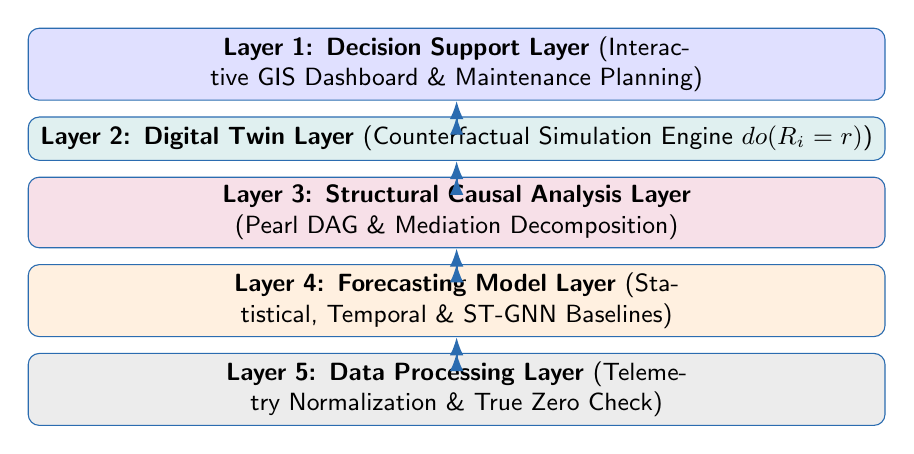
\begin{tikzpicture}[
      layerbox/.style={draw=secblue, fill=#1, text width=0.88\textwidth, align=center, rounded corners=4pt, font=\small\sffamily, minimum height=0.55cm, inner sep=3pt},
      arrowstyle/.style={Latex-Latex, thick, secblue}
    ]
      \node [layerbox=blue!12] (L1) {\textbf{Layer 1: Decision Support Layer} (Interactive GIS Dashboard \& Maintenance Planning)};
      \node [layerbox=teal!12, below=0.20cm of L1] (L2) {\textbf{Layer 2: Digital Twin Layer} (Counterfactual Simulation Engine $do(R_i=r)$)};
      \node [layerbox=purple!12, below=0.20cm of L2] (L3) {\textbf{Layer 3: Structural Causal Analysis Layer} (Pearl DAG \& Mediation Decomposition)};
      \node [layerbox=orange!12, below=0.20cm of L3] (L4) {\textbf{Layer 4: Forecasting Model Layer} (Statistical, Temporal \& ST-GNN Baselines)};
      \node [layerbox=gray!15, below=0.20cm of L4] (L5) {\textbf{Layer 5: Data Processing Layer} (Telemetry Normalization \& True Zero Check)};
      
      \draw [arrowstyle] (L5) -- (L4);
      \draw [arrowstyle] (L4) -- (L3);
      \draw [arrowstyle] (L3) -- (L2);
      \draw [arrowstyle] (L2) -- (L1);
    \end{tikzpicture}
  \end{center}
\end{frame}

% ==================== SLIDE 11: FUNCTIONAL LAYERS ====================
\begin{frame}{9. Proposed Functional Layers}
  \begin{description}
    \item[Data Processing Layer:] Normalizes speed telemetry and evaluates spatial neighborhood velocity checks to separate real traffic dead-stops from hardware dropouts.
    \item[Forecasting Model Layer:] Manages baseline models (HA, DLinear, DCRNN, GWNet) to generate multi-horizon speed predictions and compute node error outputs.
    \item[Causal Analysis Layer:] Models causal relationships among reliability, traffic density, and topology, isolating indirect hardware attribution pathways.
    \item[Digital Twin Layer:] Provides a virtual simulation environment to evaluate counterfactual hardware maintenance scenarios ($do(R_i = 0.95)$).
    \item[Decision Support Layer:] Translates simulation outputs into interactive spatial health maps and regional equity dashboards.
  \end{description}
\end{frame}

% ==================== SLIDE 12: INFORMATION FLOW (TIKZ CORRECTED) ====================
\begin{frame}{10. Proposed Information Flow}
  \begin{center}
    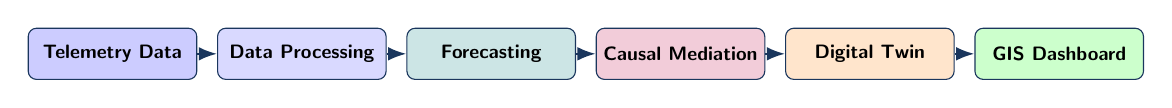
\begin{tikzpicture}[
      flowbox/.style={draw=mainblue, fill=#1, text width=2.0cm, align=center, rounded corners=3pt, font=\scriptsize\bfseries\sffamily, minimum height=0.65cm, inner sep=2pt},
      flowarrow/.style={-Latex, thick, mainblue}
    ]
      \node[flowbox=blue!20] (n1) {Telemetry Data};
      \node[flowbox=blue!15, right=0.25cm of n1] (n2) {Data Processing};
      \node[flowbox=teal!20, right=0.25cm of n2] (n3) {Forecasting};
      \node[flowbox=purple!20, right=0.25cm of n3] (n4) {Causal Mediation};
      \node[flowbox=orange!20, right=0.25cm of n4] (n5) {Digital Twin};
      \node[flowbox=green!20, right=0.25cm of n5] (n6) {GIS Dashboard};

      \draw[flowarrow] (n1) -- (n2);
      \draw[flowarrow] (n2) -- (n3);
      \draw[flowarrow] (n3) -- (n4);
      \draw[flowarrow] (n4) -- (n5);
      \draw[flowarrow] (n5) -- (n6);
    \end{tikzpicture}
  \end{center}

  \begin{block}{Sequential Feed-Forward Pipeline}
    \begin{itemize}
      \item Data Processing Layer prepares raw speed telemetry and flags dropouts.
      \item Forecasting Layer computes multi-horizon baseline predictions.
      \item Causal Analysis Layer isolates physical hardware attribution pathways.
      \item Digital Twin Layer simulates targeted virtual hardware maintenance.
      \item Decision Support Layer renders spatial equity dashboards for planning.
    \end{itemize}
  \end{block}
\end{frame}

% ==================== SLIDE 13: LITERATURE 1 ====================
\begin{frame}{11. Literature Survey: Forecasting Baselines}
  \begin{table}
    \small
    \begin{tabular}{lp{4.5cm}p{4.5cm}}
      \toprule
      \textbf{Model} & \textbf{Core Merit} & \textbf{Key Limitation} \\
      \midrule
      DCRNN [1] & Random-walk diffusion conv + GRU & Slow RNN loops; static distance graph \\
      Graph WaveNet [2] & Self-adaptive adjacency + 1D TCN & Static adaptive graph; masks dropouts \\
      STGCN [3] & 1D GLU temporal conv + ChebNet & Poor 60m stability; fixed distance matrix \\
      AGCRN [4] & Node Adaptive Parameters (NAPL) & High memory footprint; abstract embeddings \\
      GMAN [5] & Transform Attention (long-horizon) & Heavy $O(N^2)$ attention latency; neglects RSF \\
      DLinear [7] & Lightweight 1-layer trend decomposition & Discards spatial graph topology ($W_{ij}$) \\
      \bottomrule
    \end{tabular}
  \end{table}
\end{frame}

% ==================== SLIDE 14: LITERATURE 2 ====================
\begin{frame}{12. Literature Survey: Fairness, Twins \& Causality}
  \begin{table}
    \small
    \begin{tabular}{lp{4.5cm}p{4.5cm}}
      \toprule
      \textbf{Model} & \textbf{Core Merit} & \textbf{Key Limitation} \\
      \midrule
      FairTP [9] / FairSTG [10] & State-guided sampling \& mix-up & Accuracy penalty (MAE loss) \\
      SUMO [11] & Microscopic vehicle physics simulation & Manual OD tuning; no causal $do$-calculus \\
      TrafficLLM [12] & Adapted LLMs for network traffic & Analyzes cyber packets, not road sensors \\
      DTCF [13] & Rubin Potential Outcomes framework & Unidentifiable joint potential copula \\
      Plecko SFM [14] & Counterfactual mediation decomposition & Designed for static tabular data \\
      Pearl Causality [15] & Establishes Backdoor \& $do$-calculus & Purely theoretical textbook \\
      \bottomrule
    \end{tabular}
  \end{table}
\end{frame}

% ==================== SLIDE 15: LITERATURE FINDINGS ====================
\begin{frame}{13. Literature Findings \& Research Gaps}
  \begin{columns}
    \begin{column}{0.48\textwidth}
      \begin{block}{Finding 1: Global MAE Blind Spot}
        ST-GNNs optimize average loss, concealing severe regional error disparities ($\text{RSF} \ge 0.35$).
      \end{block}
      \begin{block}{Finding 2: Software Fairness Penalty}
        Observational loss re-weighting forces a trade-off against forecasting accuracy.
      \end{block}
    \end{column}
    \begin{column}{0.48\textwidth}
      \begin{block}{Finding 3: Omission of Hardware Health}
        Existing models treat physical sensor failures as software optimization targets.
      \end{block}
      \begin{block}{Finding 4: Lack of Pearl Level-3 Twins}
        Microscopic twins replay physics without causal $do$-calculus intervention capability.
      \end{block}
    \end{column}
  \end{columns}
\end{frame}

% ==================== SLIDE 16: METHODOLOGY DATA ====================
\begin{frame}{14. Proposed Methodology: Data \& Graph Construction}
  \begin{columns}
    \begin{column}{0.48\textwidth}
      \begin{block}{Dataset \& Preprocessing}
        \begin{itemize}
          \item \textbf{Dataset:} METR-LA (207 loop sensors, 5-min intervals).
          \item \textbf{Windowing:} 12 historical steps (60 min) $\to$ 12 future steps.
          \item \textbf{Normalization:} Z-score speed scaling.
        \end{itemize}
      \end{block}
    \end{column}
    \begin{column}{0.48\textwidth}
      \begin{block}{Graph Laplacian Spectral Clustering}
        \begin{itemize}
          \item \textbf{Adjacency Matrix:} Thresholded Gaussian distance kernel.
          \item \textbf{Normalized Laplacian:} Symmetric graph matrix decomposition.
          \item \textbf{Eigen-Gap Partitioning:} Maximum eigen-gap peak partitions network into spatial sub-districts ($K=13$).
        \end{itemize}
      \end{block}
    \end{column}
  \end{columns}
\end{frame}

% ==================== SLIDE 17: METHODOLOGY SENSORS ====================
\begin{frame}{15. Proposed Methodology: Disentanglement \& Reliability}
  \begin{block}{Spatial Neighborhood Disentanglement}
    Evaluates sensor speed relative to surrounding graph neighbors to separate:
    \begin{itemize}
      \item \textbf{True Zero (Real Congestion):} Speed $\le 1$ mph AND neighbors $\le 15$ mph.
      \item \textbf{Stuck-Zero (Hardware Fault):} Speed $\le 1$ mph BUT neighbors $> 15$ mph.
    \end{itemize}
  \end{block}
  
  \vspace{0.2cm}
  
  \begin{block}{Composite Hardware Reliability Index ($R_i$)}
    Combines Stuck-Zero dropout rate ($Z_i$), CUSUM cumulative calibration drift ($D_i$), and EWMA volatility spikes ($V_i$) into a standardized reliability index ($R_i \in [0, 1]$).
  \end{block}
\end{frame}

% ==================== SLIDE 18: METHODOLOGY CAUSAL & TWIN (TIKZ CORRECTED) ====================
\begin{frame}{16. Proposed Methodology: Causal DAG \& Digital Twin}
  \begin{columns}
    \begin{column}{0.45\textwidth}
      \begin{block}{Pearl Level-3 Causal DAG}
        \centering
        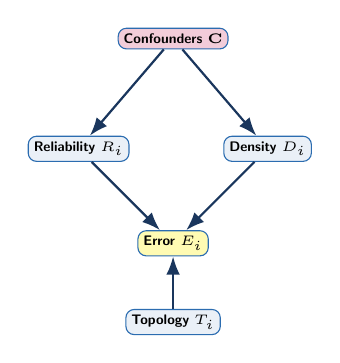
\begin{tikzpicture}[
          dagnode/.style={draw=secblue, fill=secblue!10, shape=rectangle, rounded corners=3pt, font=\tiny\bfseries\sffamily, inner sep=2pt},
          dagarrow/.style={-Latex, thick, mainblue}
        ]
          \node[dagnode, fill=purple!20] (C) at (1.2, 1.4) {Confounders $\mathbf{C}$};
          \node[dagnode] (R) at (0, 0) {Reliability $R_i$};
          \node[dagnode] (D) at (2.4, 0) {Density $D_i$};
          \node[dagnode, fill=yellow!30] (E) at (1.2, -1.2) {Error $E_i$};
          \node[dagnode] (T) at (1.2, -2.2) {Topology $T_i$};
          
          \draw[dagarrow] (C) -- (R);
          \draw[dagarrow] (C) -- (D);
          \draw[dagarrow] (R) -- (E);
          \draw[dagarrow] (D) -- (E);
          \draw[dagarrow] (T) -- (E);
        \end{tikzpicture}
      \end{block}
    \end{column}
    \begin{column}{0.52\textwidth}
      \begin{block}{Virtual Interventional Digital Twin}
        \begin{itemize}
          \item Backdoor adjustment conditions on $\{\text{road\_type}, \text{traffic\_regime}\}$.
          \item Simulates targeted physical hardware repair queries ($do(R_i = r_{\text{target}})$) virtually.
          \item Evaluates Regional Static Fairness (RSF) and accuracy metrics (MAE, RMSE, MAPE).
        \end{itemize}
      \end{block}
    \end{column}
  \end{columns}
\end{frame}

% ==================== SLIDE 19: AUTOMATED MULTI-PAGE REFERENCES (LARGE TEXT) ====================
\begin{frame}[allowframebreaks]{17. References}
  \footnotesize
  \begin{enumerate}
    \item Li, Y., Yu, R., Shahabi, C., \& Liu, Y. (2018). Diffusion convolutional recurrent neural network: Data-driven traffic forecasting. \textit{In Proceedings of ICLR 2018}, 1–16.
    
    \item Wu, Z., Pan, S., Long, G., Jiang, J., \& Zhang, C. (2019). Graph WaveNet for deep spatial-temporal graph modeling. \textit{In Proceedings of IJCAI 2019}, 1907–1913.
    
    \item Yu, B., Yin, H., \& Zhu, Z. (2018). Spatio-temporal graph convolutional networks: A deep learning framework for traffic forecasting. \textit{In Proceedings of IJCAI 2018}, 3634–3640.
    
    \item Bai, L., Yao, L., Li, C., Wang, X., \& Wang, C. (2020). Adaptive graph convolutional recurrent network for traffic forecasting. \textit{Advances in NeurIPS 2020}, 33, 17804–17815.
    
    \item Zheng, C., Fan, X., Wang, C., \& Zheng, J. (2020). GMAN: A graph multi-attention network for traffic prediction. \textit{In Proceedings of AAAI 2020}, 34(01), 1234–1241.
    
    \item Fu, M., Zhou, W., \& Chen, Z. (2021). Bayesian graph convolutional network for traffic prediction. \textit{IEEE Transactions on Intelligent Transportation Systems}, 22(11), 7120–7131.
    
    \item Zeng, A., Chen, M., Zhang, L., \& Xu, Q. (2023). Are transformers effective for time series forecasting?. \textit{In Proceedings of AAAI 2023}, 37(9), 11121–11128.
    
    \item Kwak, J., Li, D., \& Geroliminis, N. (2024). A two-level resolution neural network with enhanced interpretability for freeway traffic forecasting. \textit{Scientific Reports}, 14, Article 31624.
    
    \item Xia, J., Yang, Y., Shen, J., Wang, S., \& Cao, J. (2025). FairTP: A prolonged fairness framework for traffic prediction. \textit{In Proceedings of AAAI 2025}.
    
    \item Lin, G., Zhou, Z., Huang, Q., Yang, K., Cheng, S., \& Wang, Y. (2025). FairSTG: Countering performance heterogeneity via collaborative sample-level optimization. \textit{IEEE Transactions on Mobile Computing}, 24(5), 1102–1115.
    
    \item Lopez, P. A., Behrisch, M., Bieker-Walz, L., Erdmann, J., Flötteröd, Y. P., Hilbrich, R., Lücken, L., Rummel, J., Wagner, P., \& Wießner, E. (2018). Microscopic traffic simulation using SUMO. \textit{In Proceedings of IEEE ITSC 2018}, 2575–2582.
    
    \item Cui, T., Lin, X., Li, S., Chen, M., Yin, Q., Li, Q., \& Xu, K. (2025). TrafficLLM: Enhancing large language models for network traffic analysis with generic traffic representation. \textit{IEEE Transactions on Knowledge and Data Engineering}, 37(2), 889–901.
    
    \item Laudy, O. (2026). The Digital Twin counterfactual framework: A validation architecture for simulated potential outcomes. \textit{arXiv preprint arXiv:2604.01325v1}, 1–28.
    
    \item Plecko, D., \& Bareinboim, E. (2024). Causal fairness analysis: Definitions, task decompositions, and algorithms. \textit{Journal of Machine Learning Research}, 25(102), 1–84.
    
    \item Pearl, J. (2009). \textit{Causality: Models, reasoning and inference} (2nd ed.). Cambridge University Press.
  \end{enumerate}
\end{frame}

% ==================== SLIDE 20: CONCLUSION ====================
\begin{frame}{18. Conclusion \& Proposal Summary}
  \begin{block}{Summary of Proposed Dissertation Contribution}
    The proposed Structural Causal Digital Twin framework establishes the first Pearl Level-3 interventional paradigm for spatiotemporal traffic GNNs, achieving regional static fairness remediation without sacrificing overall forecasting accuracy.
  \end{block}

  \vspace{0.4cm}

  \centering
  \Large \textbf{Thank You!} \\
  \vspace{0.2cm}
  \small Questions \& Answers / Technical Proposal Review
\end{frame}

\end{document}
